\chapter{Web Server}
\label{sec:webserver}

\author{Nico Leidenfrost}
%
To make a web application accessible to a user, there needs to be a web server which serves the files to the web browser of the user. In the case of GRAMOC, Nginx was chosen to be used as a web server \autocite{nginx}.

A web server is a server dedicated to provide information, web sites or web applications. To achieve this goal the web server first transmits the files needed to run the web application and then sends information whenever it is requested. In this project, Nginx was selected to be utilized as a web server \autocite{nginx}.

\section{Apache}
Apache HTTP Server was first launched in 1995 \autocite{apache}. It gained a lot of popularity very quick and since April 1996 it is the most used Web Server of active websites. Apache's approach on how to handle incoming connections is quite simple, for each connection there is one thread. This can lead to problems when a lot of client are trying to connect to the server at the same time. Because, especially on not so powerful servers, the maximum amount of clients can be reached rather quickly if there is only one server available. Apache consists of a core module and many dynamically loadable modules. These modules provide various features like:

\begin{itemize}
    \item Support for various programming languages
    \item URL rewrite
    \item Proxy functionality
    \item SSL support
    \item Authentication utilities
\end{itemize}

And many more modules with their own features are available. This module system gives Apache a lot of power in terms of flexibility, because there is no need to use other systems as Apache itself to provide these features.

\section{Nginx}
Nginx is a lightweight web server that was initially created to solve the ``c10K'' problem. The goal of this challenge was to create a web server that is able to handle ten thousand concurrent client connections at once. To achieve this goal, the main difference between Nginx and its competitors is that Nginx handles client connections asynchronously instead of synchronously. Nginx is also event driven and single threaded. This means that there is only one thread running and not one thread per connection. In GRAMOC, Nginx is used to provide only the core features of a web server. This means to provide the static web application content and basic routing between the web server and the Node server. Any other functionality will be passed to components that can handle the specific tasks. Nginx was chosen over Apache because of its lightweight and speed. This is mainly achieved through passing on tasks to other programs and not trying to handle everything on its own like Apache does.

\section{Apache vs Nginx}
According to Upguard, a cyber security company, Nginx is about 4.2 times faster than Apache. The main reason for this is the single threaded, asynchronous approach of Nginx \autocite{UpguardAvN}.
Apache however contains a much larger feature set and better support, because of the fact that Apache is a lot older than Nginx. The smaller feature set of Nginx can be seen as a disadvantage, but also as an advantage. Less features are usually a clear disadvantage, but on the other hand if there are less features available, the system is much more lightweight. Thats one of the main reasons why Nginx was chosen in GRAMOC. Due to this lightweight, Nginx can operate also on systems with less computing power, like the Raspberry Pi in the case of GRAMOC.
In terms of popularity Apache is at the time of writing twice as much used in Web Server development as Nginx. These figures originate from the \textit{February 2018 Web Server Survey} conducted by Netcraft and are shown in figure \ref{fig:netcraft_survey} \autocite{netcraft_survey}.

\begin{figure}[H]
    \centering
    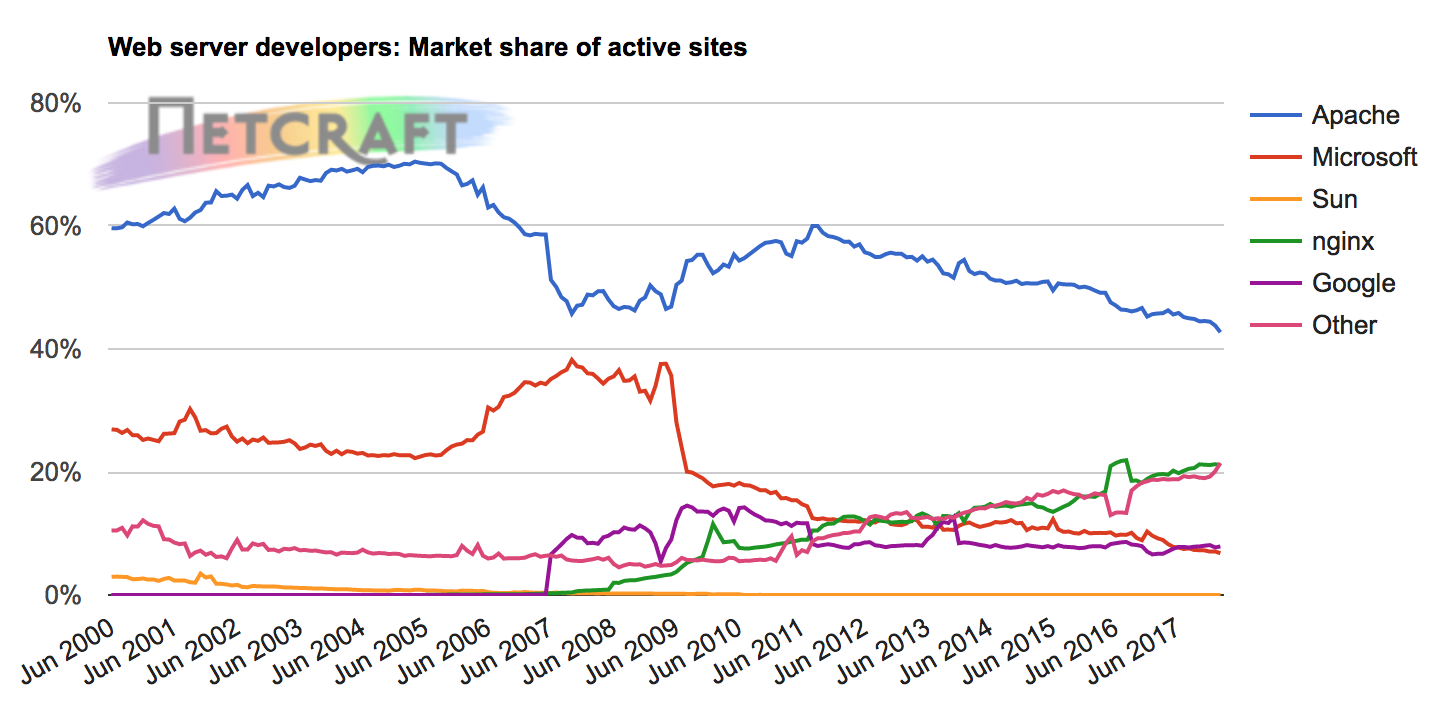
\includegraphics[width=15cm,keepaspectratio]{netcraft_survey}
    \caption{Survey results about most used Web Servers in currently active websites}
    \label{fig:netcraft_survey}
\end{figure}

These results show that Apache is still the number one Web Server with 42.72 percent market share. Number two with 21.13 percent is Nginx. The trend shows that Nginx is gaining more and more popularity as Apache slowly looses its market share. Below these two main competitors there is Google's in house developed Web Server, which they use for their own services, and Microsoft's IIS.

\section{Node.js}
\label{subsec:nodejs}
Node.js is an asynchronous event driven JavaScript runtime, designed to build network applications \autocite{Node}. The built-in HTTP module can be used to create a web server based on Node. This module is used to utilize communication over the HTTP protocol. In terms of GRAMOC the sensor data is received via a UDP connection and then transmitted over HTTP to the web application. Therefore, the primary function of the Node server is to receive data which is emitted by the Filtering and Preprocessing Layer (FAPS) and forward it, to the web application via WebSockets implemented through the ``socket.io'' library \autocite{socketio}. In order to use socket.io the HTTP module in combination with the express framework must be used.

Another function of the Node server is to provide an application programming interface(API) to request the saved sensor data. This is achieved by using the express framework. This API is needed to display historical sensor data within the GRAMOC web application.

\section{Express}
Express is a minimal and flexible web application framework to be used with Node.js. It is based on the HTTP module, which is a part of the standard library of Node.js and its main focus is to manage the routing tasks associated with the running HTTP server. So Express is just a layer on top of a web server, but not a web server itself.

\section{socket.io}
\label{subsec:socketio}
socket.io is a JavsScript library that implements real-time communication via WebSockets. This library was chosen because it aims to make real-time applications possible in every browser and can be used in a Node.js application. Since GRAMOC was built with the intent of delivering sensor data in real-time to the user, socket.io helped a lot in the step of implementing real-time communication.

\section{REST API}
GRAMOC also saves the incoming sensor data beside plotting it. This data is especially useful to create statistics or if a user wants to inspect the sensor data of a certain point of time. How the data is saved is further explained in chapter \nameref{ch:faps-save}. To make the stored sensor data available to users, a REST API(Application Programming Interface) was implemented.
REST means \textit{REpresentational State Transfer}, which is an architectural style. To call an API RESTful it needs to satisfy a number of constraints \autocite{rest}:

\begin{itemize}
    \item Client-Server
    \item Stateless
    \item Cache
    \item Uniform Interface
    \item Layered System
    \item Code-On-Demand
\end{itemize}

\subsection{Client-Server}
The Client-Server constraint simply says that there needs to be at least one server, which is able to provide data to a number of clients. This is useful, because with the separation of server and client they can be developed independently to each other. This can result in better scalability of each component.

\subsection{Stateless}
A stateless system can not store data from clients to use this data in future requests. Each request must contain enough information, so that the server is able to send an appropriate response. This constraint leads also to improved performance as the server does not need to store any contextual data about clients and is therefore able to process multiple requests faster.

\subsection{Cache}
A response must be explicitly marked as cacheable or non-cacheable. If a response is marked as cachable, it can be reused for future equivalent requests. This is useful if such cached information can be reused at least one time, because then the client can simply use the cached data instead of sending a new request to the server every time.

\subsection{Uniform Interface}
A REST API should have a standardized uniform interface in order to maintain the simplicity of interactions. A resource in a system should only have one logical URI.


\subsection{Layered System}
In a layered system, every component can access only the layer next to it. This removes a lot of complexity from the system, as a component just needs to interact with its neighbors.

\subsection{Code-On-Demand}
The last constraint within the REST architecture is the Code-On-Demand constraint which is only optional. It allows an API to send executable code to the clients to extend their set of features. This is used to create simple clients which can be dynamically extended after deployment.

\subsection{Implementation}
In the GRAMOC REST API are only GET routes, as there is no need to change or modify data. The GET routes are implemented as in the following table \ref{tab:get_routes}

\begin{table}[H]
    \centering
    \begin{tabular}{| l | l |}
    \hline
    \textbf{Route} & \textbf{Response} \\ \hline
    /files & returns a list of files within the data directory \\ \hline
    /files/:file/data & returns the data of each dataset inside a file \\ \hline
    /files/:file/datasets & returns a list of datasets stored inside a file \\ \hline
    /files/:file/datasets/:id & returns the data of a specific dataset \\
    \hline
    \end{tabular}
    \caption{GET request routes of the REST API used in GRAMOC}
    \label{tab:get_routes}
\end{table}

The files are all stored in a specific directory from which the API can read. Inside these files there are datasets, which represent time points. With this structure it is possible to request the data from a specific timespan.
